\documentclass[12pt]{beamer}
\usepackage{amsmath,amssymb,caption,float,hyperref,minted}
\usepackage[ruled,vlined]{algorithm2e}
\usepackage[utf8]{inputenc}
\usepackage[english]{babel}
\usepackage[backend=bibtex]{biblatex}
\addbibresource{p2pre.bib}
\definecolor{bg}{rgb}{0.95,0.95,0.95}
\hypersetup{
    colorlinks=true,
    linkcolor=blue,
    filecolor=blue,      
    urlcolor=blue,
    citecolor=cyan,
}
\usemintedstyle{emacs}
\usetheme{Madrid}
\setbeamercolor{normal text}{bg=black!10}

\SetKwInOut{Input}{Input}
\SetKwInOut{Output}{Output}
\SetKwProg{Fn}{Function}{\string:}{end}
\SetKwFunction{parse}{parse}

\begin{document}
\title{Git Collaboration}
\subtitle{VE482 Project2 Presentation}
\author[Group 11]{Group 11, Yihua Liu, Yu Xiao}
\institute{UM-SJTU Joint Institute}
\date{\today}
\begin{frame}
    \titlepage
\end{frame}

\section{Collaboration Techniques}
\begin{frame}{Start from a small group of 4 members}
    1. Owner-Contributor Mode - a centralized approach\\
    This mode applies to the case that one main contributor does most of the work and other contributors serve as assistants of the main contributor to do minor changes, modifications, or patches.
    \begin{itemize}
        \item The main contributor also the team leader creates a repository and a \texttt{main} branch as the Owner. Usually, she or he does all of her or his work on the \texttt{main} branch and is responsible to review and merge other contributors' pull requests.
        \item Usually, the members directly fork the repository, make changes on their own branches, create pull requests, and wait for the main contributor to merge their changes.
        \item If the repository has grew very large and a patch is complex, the owner may create a \texttt{develop} branch. They will work on \texttt{develop} normally, and merge \texttt{develop} to \texttt{main} periodically.
    \end{itemize}
\end{frame}
\begin{frame}{Start from a small group of 4 members}
    2. Team Members Mode - a decentralized approach\\
    This mode applies to the case that the 4 contributors are a developer team. Our Project 2 uses this method. All the members have the same rights to the repository.
    \begin{itemize}
        \item The 4 members may be divided into 2 pairs. Each pair maintains its own branches for different tasks.
        \item When a task is finished, one pair creates a pull request. The branch would be merged to \texttt{main} only if both pairs (all the 4 members) permit.
    \end{itemize}
    3. Owner-Collaborator Mode\\
    This mode is somewhere in between. Collaborators also have the rights to merge pull requests, so they can work on their own branches and merge them without others' permissions.
\end{frame}
\begin{frame}{When the group grows to 10}
    \begin{alertblock}{Problem}
        Merge conflicts may happen frequently.
    \end{alertblock}
    \begin{block}{Solution}
    \begin{itemize}
        \item Always \texttt{git pull} first before committing to public branches.
        \item Use \texttt{git rebase <branch\_name>} to detect merge conflicts before merging and resolve conflicts locally.
        \item Use more branches.
    \end{itemize}
    \end{block}
    Number of branches is more related to the size/complexity of the repositories rather than number of contributors. For example, \href{https://github.com/996icu/996.ICU}{996.ICU} (607 contributors) and \href{https://github.com/ohmyzsh/ohmyzsh}{ohmyzsh} (1930 contributors) only have the \texttt{main} branch. However, to use multiple branches is always better than to use the single \texttt{main} branch.
\end{frame}

\begin{frame}{When the group grows to 10 - Organizations}
    Organizations are flexible. They can be as small as 10 members, or as large as 100,000 members. For example, \href{https://github.com/EpicGames}{Epic Games} has 365.4k members, and \href{https://github.com/NVIDIAGameWorks}{NVIDIA GameWorks} has 24.6k members.
    \begin{block}{Question}
        Why to use organizations?
    \end{block}
    On the contrary to \textbf{user repositories} mentioned before, organizations work on \textbf{group repositories}.% We can manage manage access and visibility of group repositories.\\
\end{frame}

\begin{frame}{When the group grows to 10 - Teams}
    \begin{figure}[H]
        \centering
        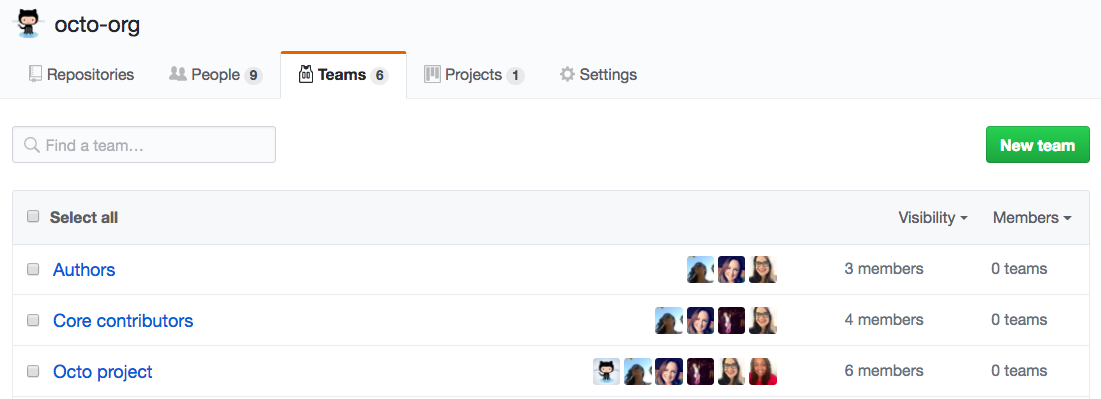
\includegraphics[width=0.8\textwidth]{org-list-of-teams.png}
    \end{figure}
    Teams are groups of organization members that reflect your company or group's structure with cascading access permissions and mentions.
\end{frame}

\begin{frame}{When the group grows to 10 - Teams}
    \begin{figure}[H]
        \centering
        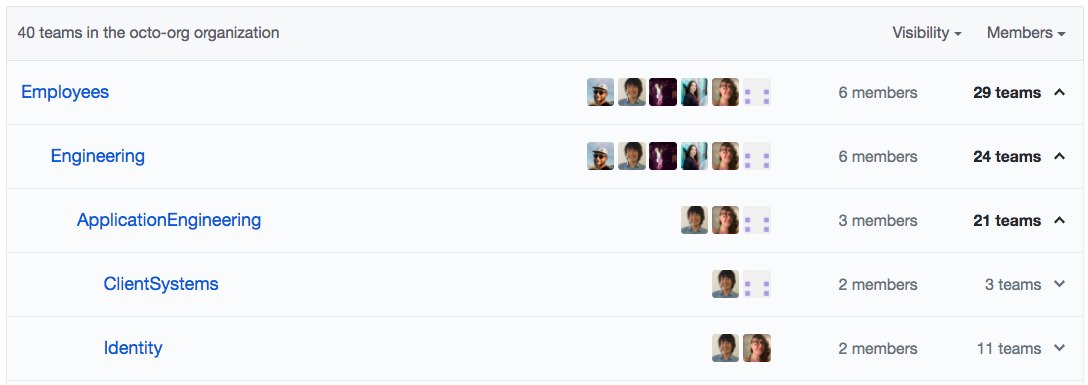
\includegraphics[width=0.6\textwidth]{nested-teams-eng-example.png}
    \end{figure}
    \begin{figure}[H]
        \centering
        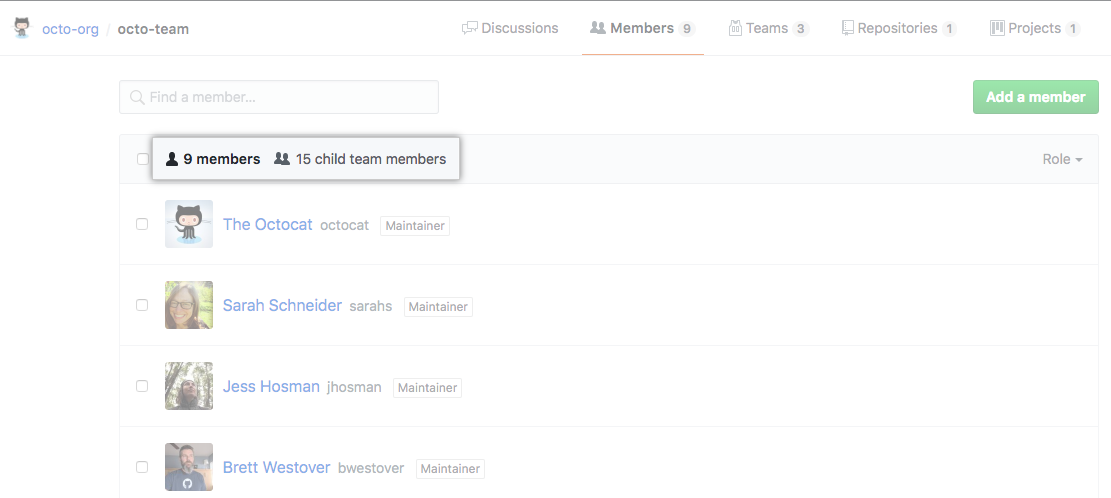
\includegraphics[width=0.6\textwidth]{team-and-subteam-members.png}
    \end{figure}
    You can even create nested teams \cite{githubdoc}.
\end{frame}

\begin{frame}{When the group grows into 100 or even 1,000 developers}
    4. Owner-Collaborator-Contributor Mode
    \begin{itemize}
        \item The owner and the collaborators maintain the repository together as the core developer group. They are responsible for reviewing and merging pull requests. The core developer group will discuss any major changes by mailing lists.
        \item Other developers serve as contributors. They develop their own branches and create pull requests. They can discuss by IRC channels (popular servers include \texttt{freenode} and \texttt{libera}), Gitter rooms, Google Group, GitHub issue and discussion pages etc.
        \item More protected branches are introduced for version control.
    \end{itemize}
    5. Owner-Member Mode -- Organization\\
    Epic Games and NVIDIA GameWorks adapts this mode. Developers must register as a group member to view and contribute to the group repositories.
\end{frame}

\begin{frame}[fragile]{Public Project over Email}
Many old, large projects accept patches via a developer mailing list \cite{gitbook}.
    \begin{minted}[frame=single,bgcolor=bg,breaklines,linenos,fontsize=\scriptsize]{text}
$ git checkout -b topicA
  ... work ...
$ git commit
  ... work ...
$ git format-patch -M origin/master
0001-add-limit-to-log-function.patch
0002-increase-log-output-to-30-from-25.patch
$ cat 0001-add-limit-to-log-function.patch
From 330090432754092d704da8e76ca5c05c198e71a8 Mon Sep 17 00:00:00 2001
From: Jessica Smith <jessica@example.com>
Date: Sun, 6 Apr 2008 10:17:23 -0700
Subject: [PATCH 1/2] Add limit to log function

Limit log functionality to the first 20

---
    \end{minted}
\end{frame}

\begin{frame}[fragile]{Public Project over Email}
    Edit \texttt{~/.gitconfig}:
    \begin{minted}[frame=single,bgcolor=bg,breaklines,linenos,fontsize=\scriptsize]{text}
[imap]
  folder = "[Gmail]/Drafts"
  host = imaps://imap.gmail.com
  user = user@gmail.com
  pass = YX]8g76G_2^sFbd
  port = 993
  sslverify = false
[sendemail]
  smtpencryption = tls
  smtpserver = smtp.gmail.com
  smtpuser = user@gmail.com
  smtpserverport = 587
    \end{minted}
\end{frame}

\begin{frame}[fragile]{Public Project over Email}
    \begin{minted}[frame=single,bgcolor=bg,breaklines,linenos,fontsize=\scriptsize]{text}
$ cat *.patch |git imap-send
Resolving imap.gmail.com... ok
Connecting to [74.125.142.109]:993... ok
Logging in...
sending 2 messages
100% (2/2) done

(mbox) Adding cc: Jessica Smith <jessica@example.com> from
  \line 'From: Jessica Smith <jessica@example.com>'
OK. Log says:
Sendmail: /usr/sbin/sendmail -i jessica@example.com
From: Jessica Smith <jessica@example.com>
To: jessica@example.com
Subject: [PATCH 1/2] Add limit to log function
Date: Sat, 30 May 2009 13:29:15 -0700
Message-Id: <1243715356-61726-1-git-send-email-jessica@example.com>
X-Mailer: git-send-email 1.6.2.rc1.20.g8c5b.dirty
In-Reply-To: <y>
References: <y>

Result: OK
    \end{minted}
\end{frame}

\begin{frame}{Large-Scale Group Work}
    In case of unlimited contributors, the general workflow for common contributors will be:
    \begin{itemize}
        \item Fork the target repository to one's own account.
        \item Clone the forked repository to the local machine.
        \item Create a new branch for a topic and make changes.
        \item Commit the changes to the forked repository.
        \item Create a pull request.
        \item Make any requested changes.
        \item Pull request approved.
    \end{itemize}
\end{frame}
\begin{frame}{Pull Request: Status Check}
    Pull request is the most important part during collaboration. Normally, this part requires one reviewer to check the committed code manually. If you are using Github, then there are some useful tools that might be helpful.
    \begin{itemize}
        \item The owner can set status checks for the repository.
    \end{itemize}
    \begin{figure}
        \centering
        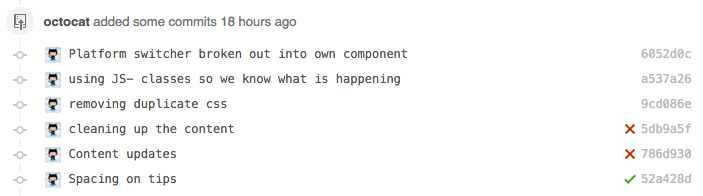
\includegraphics[width=0.8\linewidth]{commit-list-statuses.png}
        \label{fig:commit-list-statuses}
    \end{figure}
    \begin{itemize}
        \item \textit{pending}, \textit{passing}, or \textit{failing} state of status checks will be shown next to each commit in the pull request.
    \end{itemize}
\end{frame}
\begin{frame}{Pull Request: Github Bot}
    \begin{itemize}
        \item The owner of the repository can also deploy a Github Bot (Github App) to help to do the code quality check.
    \end{itemize}
    \begin{figure}
        \centering
        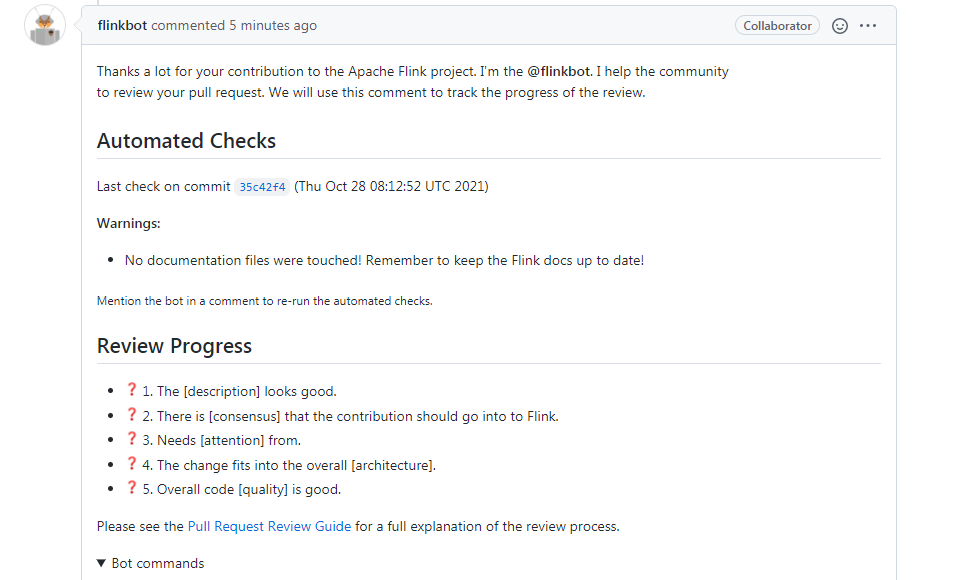
\includegraphics[width=0.8\linewidth]{github_bot_apache_flink.png}
        \label{fig:github_bot_apache_flink}
    \end{figure}
\end{frame}
\begin{frame}{Secondary Channels}
    Some big projects are not totally based on online development platforms like Github (e.g. linux).
    \begin{figure}
        \centering
        \includegraphics[width=0.8\linewidth]{linux.png}
        \label{fig:linux}
    \end{figure}
    Some universities also have their own git server that serves as online development platform.
\end{frame}
\section{Reference}
\begin{frame}{Reference}
    \printbibliography
\end{frame}
\section{}
\begin{frame}{}
    \begin{center}
        \Huge Thanks!
    \end{center}
\end{frame}
\end{document}
